\section{Lecture 11: Advanced Topics on Pattern Discovery}

% --
\subsection{Frequent Pattern Mining in Data Streams}

\subsubsection{Lossy Counting Algorithm}
\begin{figure}[H]
    \centering
    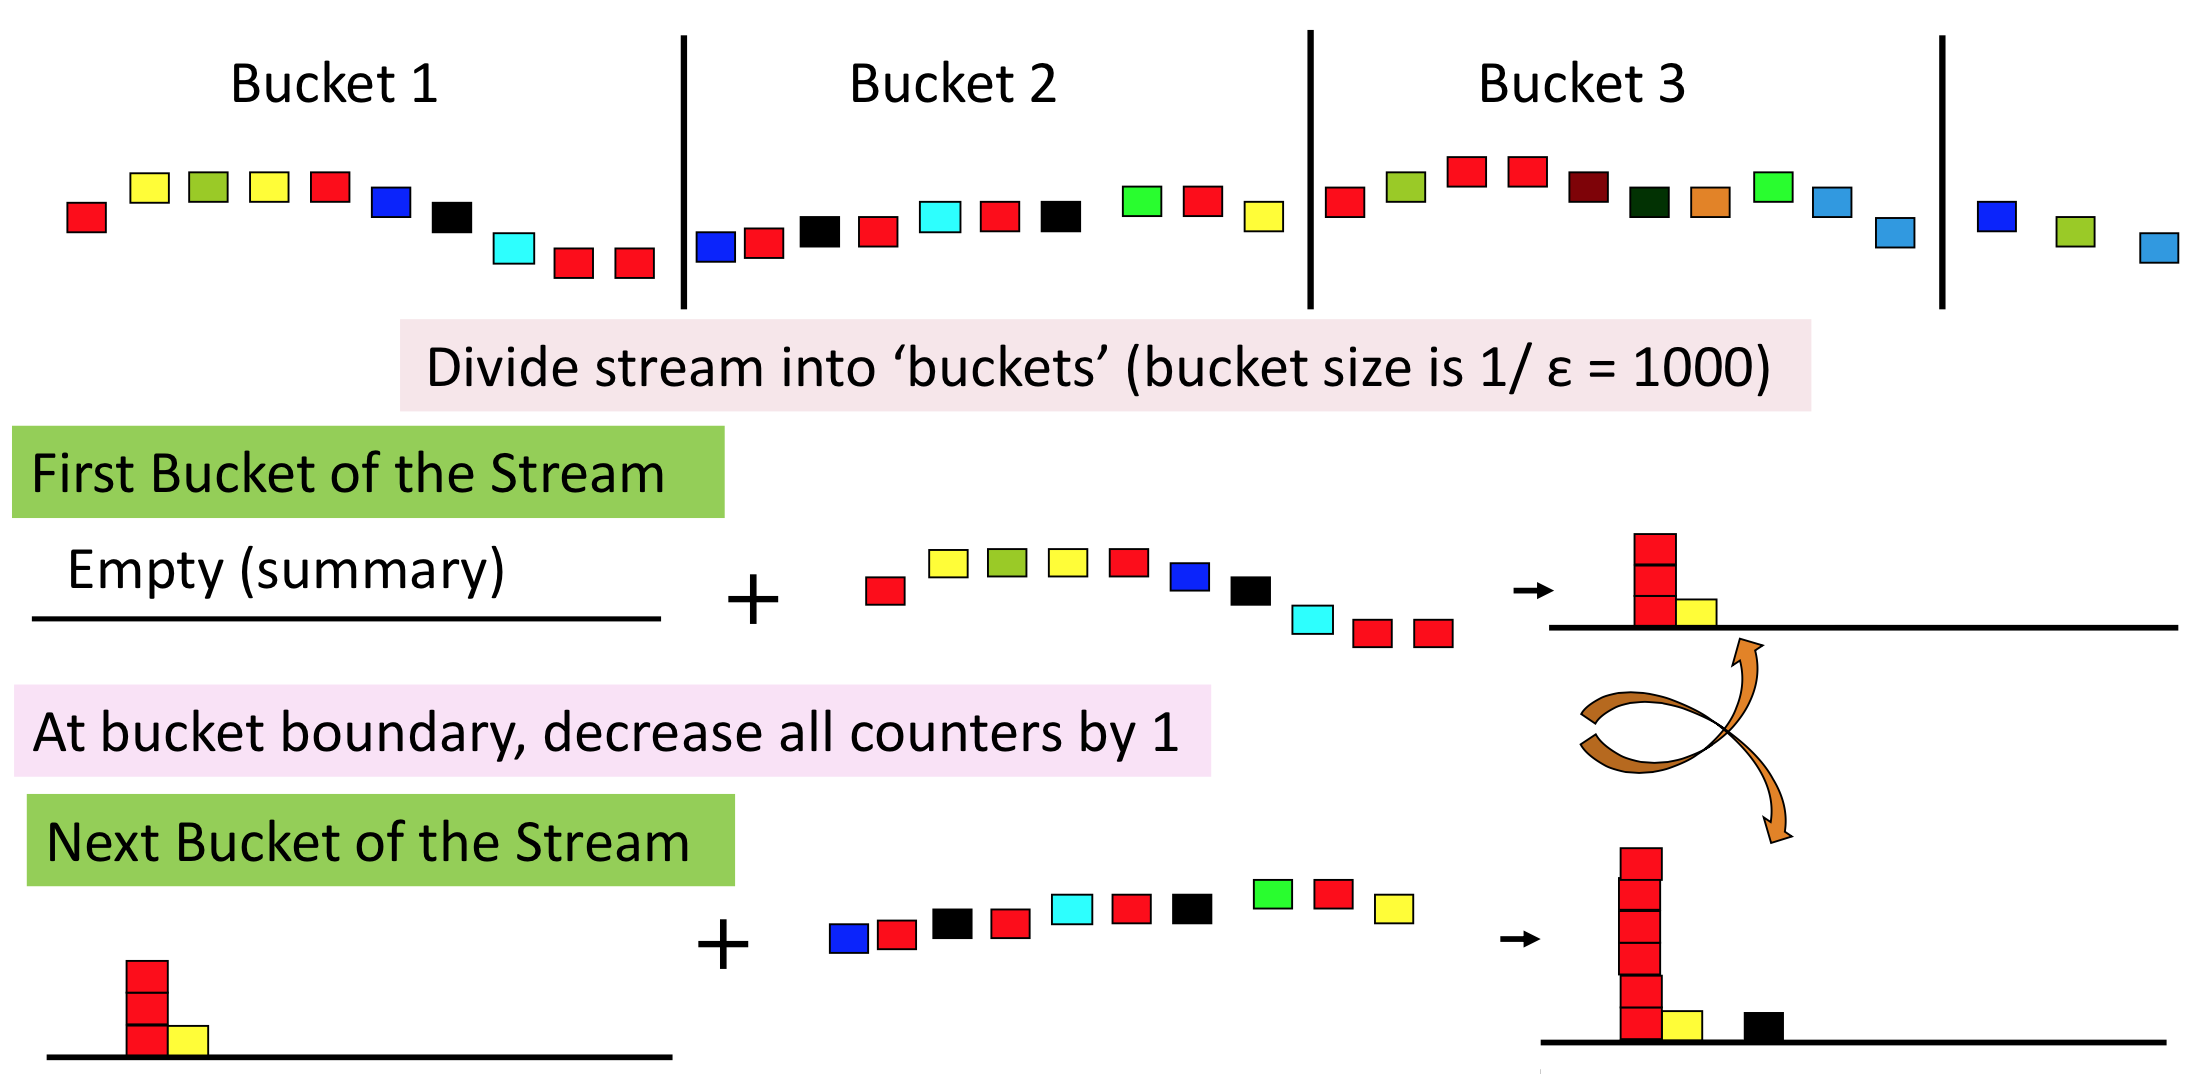
\includegraphics[width=\linewidth]{LossyCountingAlgorithm.png}
    \caption{Lossy Counting Algorithm}
\end{figure}

\newpage
Given: 
\begin{itemize}
\item support threshold = $\sigma$
\item error threshold = $\varepsilon$
\item stream length = $N$
\end{itemize}

Output: items with frequency counts exceeding $(\sigma – \varepsilon) \times N$


\begin{equation*}
\textit{frequency count error} \leqslant \textit{number of buckets} = \frac{N}{\textit{bucket size}} = \frac{N}{1/\varepsilon} = \varepsilon N
\end{equation*}

Approximation guarantee:
\begin{itemize}
\item  No false negatives
\item  False positives have true frequency count at least $(\sigma – \varepsilon) \times N$
\item Frequency count underestimated by at most $\varepsilon N$
\end{itemize}

\subsubsection{Recommended Readings}
\begin{itemize}
\item G. Manku and R. Motwani, <<Approximate Frequency Counts over Data
Streams>>, VLDB’02
\item A. Metwally, D. Agrawal, and A. El Abbadi, <<Efficient Computation of Frequent and Top-k Elements in Data Streams>>, ICDT'05
\end{itemize}

%--
\subsection{Spatiotemporal and Trajectory Pattern Mining}
\subsubsection{Mining Relative Movement Patterns}
\begin{itemize}
\item \textbf{Flock}: At least m entities are within a circular region of radius r and move in the same direction
\item \textbf{Convoy}: Uses density-based clustering at each timestamp; no need to be a rigid circle
\item \textbf{Swarm}: Moving objects may not be close to each other for all the consecutive time stamps
\end{itemize}


\subsubsection{Recommended Readings}
\begin{itemize}
\item Y. Huang, S. Shekhar, H. Xiong, Discovering colocation patterns from spatial data sets: A general approach, IEEE Trans. on Knowledge and Data Engineering, 16(12), 2004
\item K. Koperski, J. Han, <<Discovery of Spatial Association Rules in Geographic Information Databases>>, SSD’95
\item Z. Li, B. Ding, J. Han, R. Kays, <<Swarm: Mining Relaxed Temporal Moving Object Clusters>>, VLDB’10
\item Z. Li, B. Ding, J. Han, Roland Kays, Peter Nye, <<Mining Periodic Behaviors for Moving Objects>>, KDD’10
\item C. Zhang, J. Han, L. Shou, J. Lu, T. La Porta, <<Splitter: Mining Fine-Grained Sequential Patterns in Semantic Trajectories>>, VLDB’14
\item Y. Zheng and X. Zhou, Computing with Spatial Trajectories, Springer, 2011
\end{itemize}


%--
\subsection{Pattern Discovery for Software Bug Mining}

\subsubsection{Typical Software Bug Detection Methods}
\begin{itemize}
\item Mining rules from source code
    \begin{itemize}
    \item Bugs as deviant behavior (e.g., by statistical analysis)
    \item Mining programming rules (e.g., by frequent itemset mining)
    \item Mining function precedence protocols (e.g., by frequent subsequence mining) 
    \item Revealing neglected conditions (e.g., by frequent itemset/subgraph mining)
    \end{itemize}

\item Mining rules from revision histories 
    \begin{itemize}
    \item By frequent itemset mining
    \end{itemize}

\item Mining copy-paste patterns from source code
    \begin{itemize}
    \item Find copy-paste bugs (e.g., CP-Miner [Li et al., OSDI’04])
    \item Reference: Z. Li, S. Lu, S. Myagmar, Y. Zhou, <<CP-Miner: A Tool for Finding Copy-paste and Related Bugs in Operating System Code>>, OSDI’04
    \end{itemize}
\end{itemize}

\subsubsection{Mining Copy-and-Paste Bugs}
\begin{figure}[h]
\centering
\subfigure[code with a bug]{%
  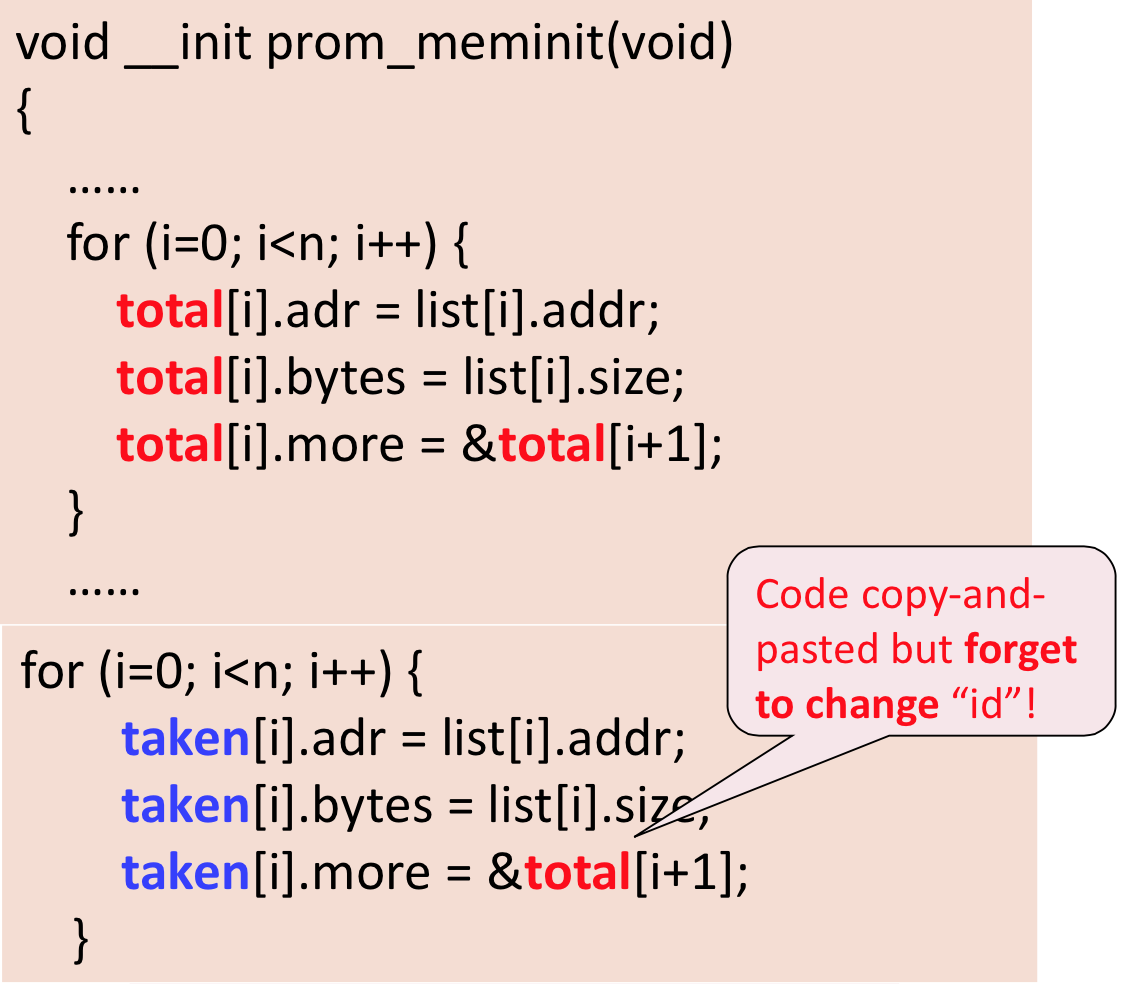
\includegraphics[width=0.45\linewidth]{CP1.png}
  \label{fig:cp1}}
\quad
\subfigure[sequence]{%
  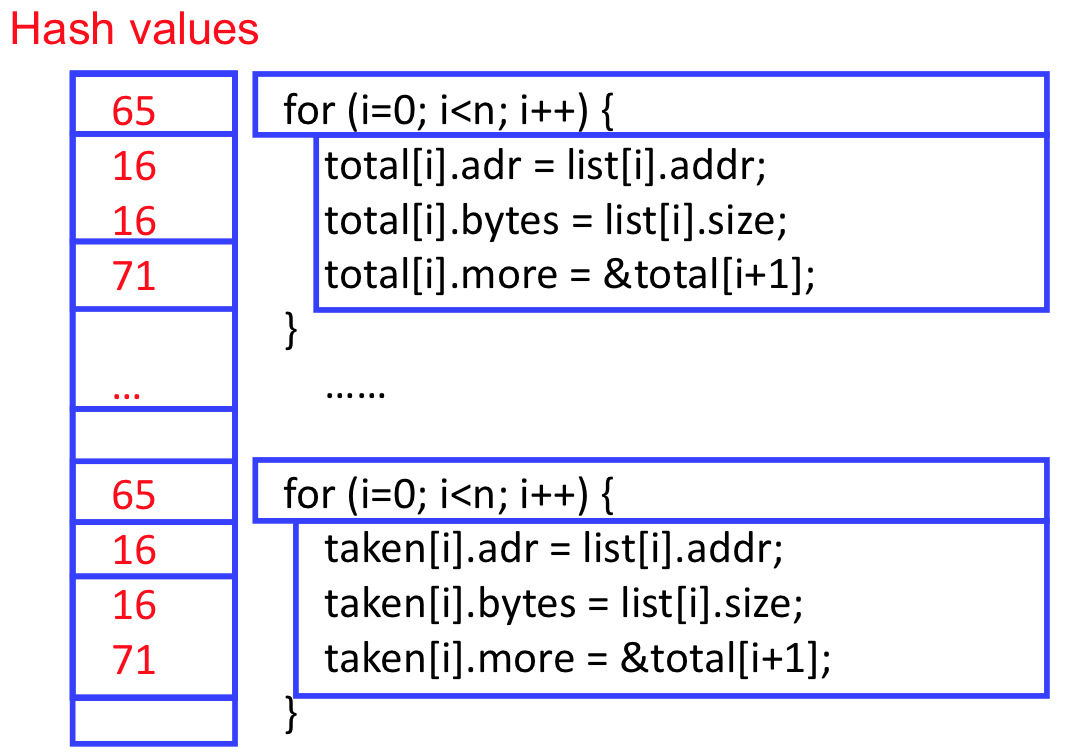
\includegraphics[width=0.45\linewidth]{CP2.png}
  \label{fig:cp2}}

\caption{Copy-and-Paste Bugs}
\label{fig:cp12}
\end{figure}

\begin{itemize}
\item Map each statement to number
\item Tokenize each component 
    \begin{itemize}
    \item Different operators, constants, keywords = different tokens
    \item Same type of identifiers = same token
    \end{itemize}
\item Program = long sequence
    \begin{itemize}
    \item Cut the long sequence by blocks.
    \end{itemize}
\end{itemize}


\begin{figure}[h]
\centering
\subfigure[Tokenize each component]{%
  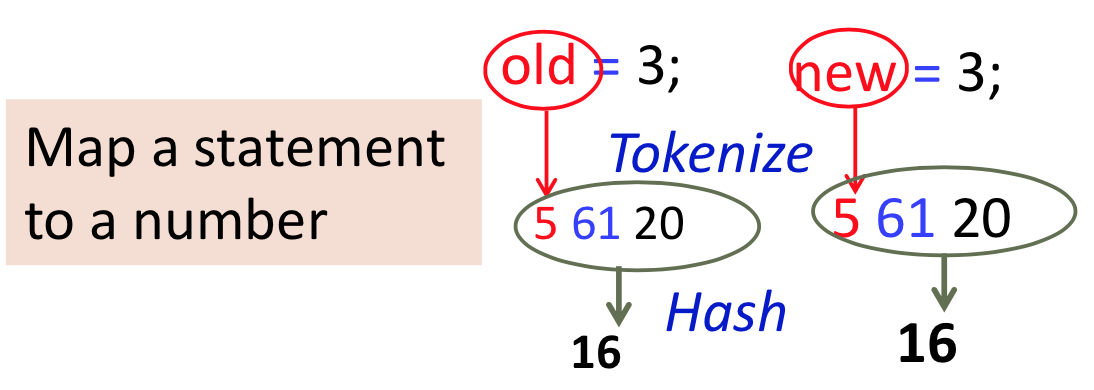
\includegraphics[width=0.65\linewidth]{CP3.png}
  \label{fig:cp3}}
\quad
\subfigure[Final sequence DB]{%
  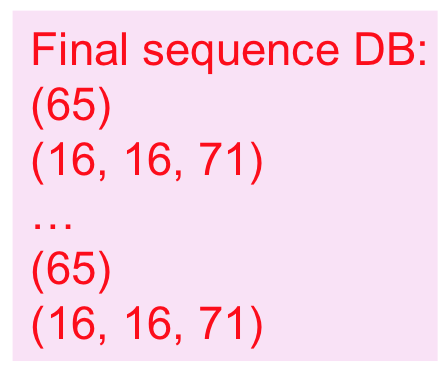
\includegraphics[width=0.25\linewidth]{CP4.png}
  \label{fig:cp4}}

\caption{Building Sequence Database from Source Code}
\label{fig:cp34}
\end{figure}


\begin{figure}[h]
\centering
\subfigure[Constrain the max gap]{%
  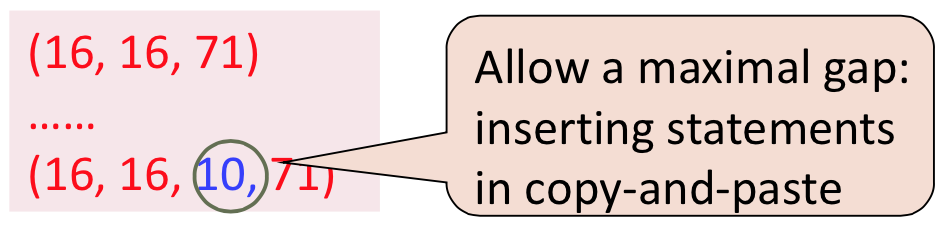
\includegraphics[width=0.45\linewidth]{CP5.png}
  \label{fig:cp5}}
\quad
\subfigure[Find conflicts]{%
  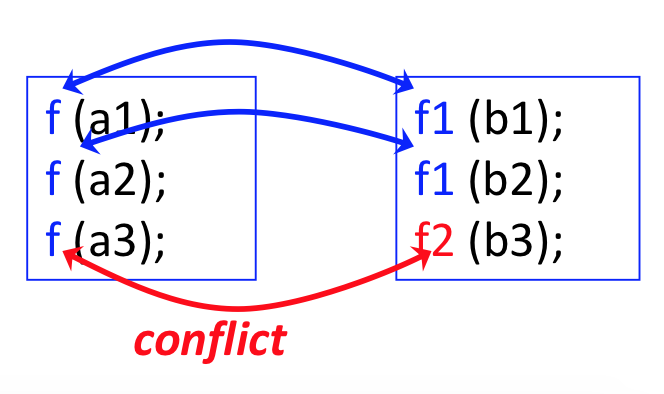
\includegraphics[width=0.45\linewidth]{CP6.png}
  \label{fig:cp6}}

\caption{Detecting <<Forget-to-Change>> Bugs}
\label{fig:cp56}
\end{figure}

\begin{itemize}
\item Modification to the sequence pattern mining algorithm
    \begin{itemize}
    \item Constrain the max gap
    \end{itemize}
    
\item Composing Larger Copy-Pasted Segments
    \begin{itemize}
    \item Combine the neighboring copy-pasted segments repeatedly
    \end{itemize}
    
\item Find conflicts: Identify names that cannot be mapped to the corresponding ones
    \begin{itemize}
    %\item E.g., 1 out of 4 <<total>> is unchanged, unchanged ratio = 0.25
    \item If $0 < \textit{unchanged ratio} < \textit{threshold}$, then report it as a bug
    \end{itemize}
\end{itemize}


%--
\subsection{Pattern Discovery for Image Analysis}
\subsubsection{Recommended Readings}
\begin{itemize}
\item Hongxing Wang, Gangqiang Zhao, Junsong Yuan, Visual pattern discovery in image and video data: a brief survey, Wiley Interdisciplinary Review: Data Mining and Knowledge Discovery 4(1): 24-37 (2014)
\item Hongxing Wang, Junsong Yuan, Ying Wu, Context-Aware Discovery of Visual Co-Occurrence Patterns. IEEE Transactions on Image Processing 23(4): 1805-1819 (2014)
\item Gangqiang Zhao, Junsong Yuan, Discovering Thematic Patterns in Videos via Cohesive Sub-graph Mining. ICDM 2011: 1260-1265
\item Junsong Yuan, Ying Wu, Ming Yang, From frequent itemsets to semantically meaningful visual patterns. KDD 2007: 864-873
\end{itemize}

%--
%\subsection{Pattern Mining and Society: Privacy Issues}
%\subsubsection{Recommended Readings}
%\begin{itemize}
%\item R. Agrawal and R. Srikant, Privacy-preserving data mining, SIGMOD'00
%\item C. C. Aggarwal and P. S. Yu, Privacy-Preserving Data Mining: Models and Algorithms, Springer, 2008
%\item C. Dwork and A. Roth. The Algorithmic Foundations of Differential Privacy. Foundations and Trends in Theoretical Computer Science. 2014
%\item A. Evfimievski, R. Srikant, R. Agrawal, and J. Gehrke. Privacy preserving mining of association rules. In KDD'02
%\item A. Gkoulalas-Divanis, J. Haritsa and M. Kantarcioglu, Privacy in Association Rule Mining, in C. Aggarwal and J. Han (eds.), Frequent Pattern Mining, Springer, 2014 (Chapter 15)
%\item N. Li, T. Li, S. Venkatasubramanian. t-closeness: Privacy beyond k-anonymity and l-diversity. ICDE'07
%\item A. Machanavajjhala, D. Kifer, J. Gehrke, M. Venkitasubramaniam, l-diversity: Privacy beyond k-
%anonymity, TKDD 2007
%\item S. Rizvi and J. Haritsa. Maintaining data privacy in association rule mining. VLDB’02
%\item J. Vaidya, C. W. Clifton and Y. M. Zhu, Privacy Preserving Data Mining, Springer, 2010
%\end{itemize}